\chapter{Distribución del producto}

Para poder usar twinX, dado que está pensado para ser accedido desde la web, tenemos que tenerlo primeramente alojado en un servidor, de modo que pueda ser accesible desde cualquier parte y con cualquier dispositivo. Hasta ahora, el desarrollo se ha llevado a cabo en un entorno de Apache \cite{apache}, mediante la ayuda de XAMPP, y  hemos podido sistematizar el funcionamiento de un \textit{webserver}. Sin embargo, para hacer las pruebas ha sido necesario alojar twinX en un servidor, al igual que para su distribución será necesario, igualmente.

\section{Despliegue (deployment)}

Dado que Amazon oferta una licencia gratuita hasta el año de graduación para estudiantes, se ha hecho uso de la herramienta AWS \cite{aws} por ello y por su gran potencial. Nosotros tan solo necesitaremos desplegar nuestra aplicación, pero hoy por hoy resulta una de las mejores alternativas, por su amplia gama de productos y su buen funcionamiento.

Para tener nuestro sitio web alojado, tras registrarnos en AWS Educate \cite{awseducate}, lo primero que tenemos que hacer es crear una instancia de máquina virtual \textbf{EC2}. Para nuestro despliegue, hemos usado una máquina con \textbf{Windows Server\textregistered 2019 Datacenter}, unos 30 GB de disco duro, 1 GB de RAM y un procesador Intel(R) Xeon(R) CPU E5-2676 v3 @ 2.40GHz con un core físico, que es lo que nos ofrece AWS en el \textit{free tier}.

Tras la creación de la instancia, se nos proporciona una clave privada que nos permitirá conectarnos al servidor. La ventaja de haber escogido Windows Server como sistema es la posibilidad de conectarnos de forma remota desde el escritorio de un ordenador con Windows y poder interaccionar como si fuera una máquina virtual local. Una vez está todo listo, aportando el archivo con la clave privada, se descarga una conexión preparada a la máquina, y con tan solo ejecutarla e introducir la clave, ya tenemos acceso a su escritorio remoto.

Una vez conectados, hemos de cambiar las preferencias del firewall (figura \ref{fig:firewall}) 

\begin{figure}
	\centering
	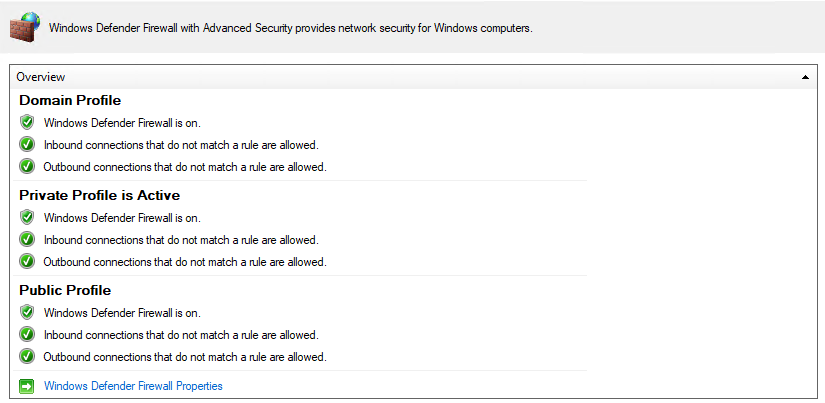
\includegraphics[width=\linewidth]{img/firewall}
	\caption{Configuración del firewall de la instancia de AWS}
	\label{fig:firewall}
\end{figure}

